% Template do Relatório Parcial e Final para o Programa Iniciação Científica da UFPR, baseado em  https://www.overleaf.com/latex/templates/modelo-pibic-ufc-itapaje/jmnnwfkhgtbw.
% Adaptado para um relatório sobre Fourier Neural Operators.
\synctex=1
\documentclass[a4paper, 12pt]{report}
\usepackage[utf8]{inputenc}
\usepackage[english]{babel} % Alterado para inglês
\usepackage[breaklinks=true, hidelinks]{hyperref}
\usepackage{breakcites}
\usepackage{ragged2e}
\usepackage{subcaption}
\usepackage{eso-pic}

\usepackage[T1]{fontenc} % Adicione isso logo abaixo de \usepackage[utf8]{inputenc}
\usepackage{helvet}

\usepackage{setspace}
\onehalfspacing % Isso define exatamente o 1,5 da ABNT

\usepackage{tikz}
\usetikzlibrary{positioning}

\usepackage{enumitem}
\usepackage{xcolor}
\usepackage{amsmath, amssymb}
\usepackage{csquotes}

% Estilo de bibliografia
% 2. Carregue o biblatex com as opções corretas para ABNT
\usepackage[
    backend=biber,     % Usa o Biber, mais moderno que o BibTeX
    style=abnt,
    maxcitenames=1,     % Citações no texto com até 3 autores, acima disso usa "et al."
    mincitenames=1      % Complemento do maxcitenames
]{biblatex}

\usepackage[acronym]{glossaries}

\newcommand\BackgroundPic{
\put(0,0){
\parbox[b][\paperheight]{\paperwidth}{
\vfill
\centering
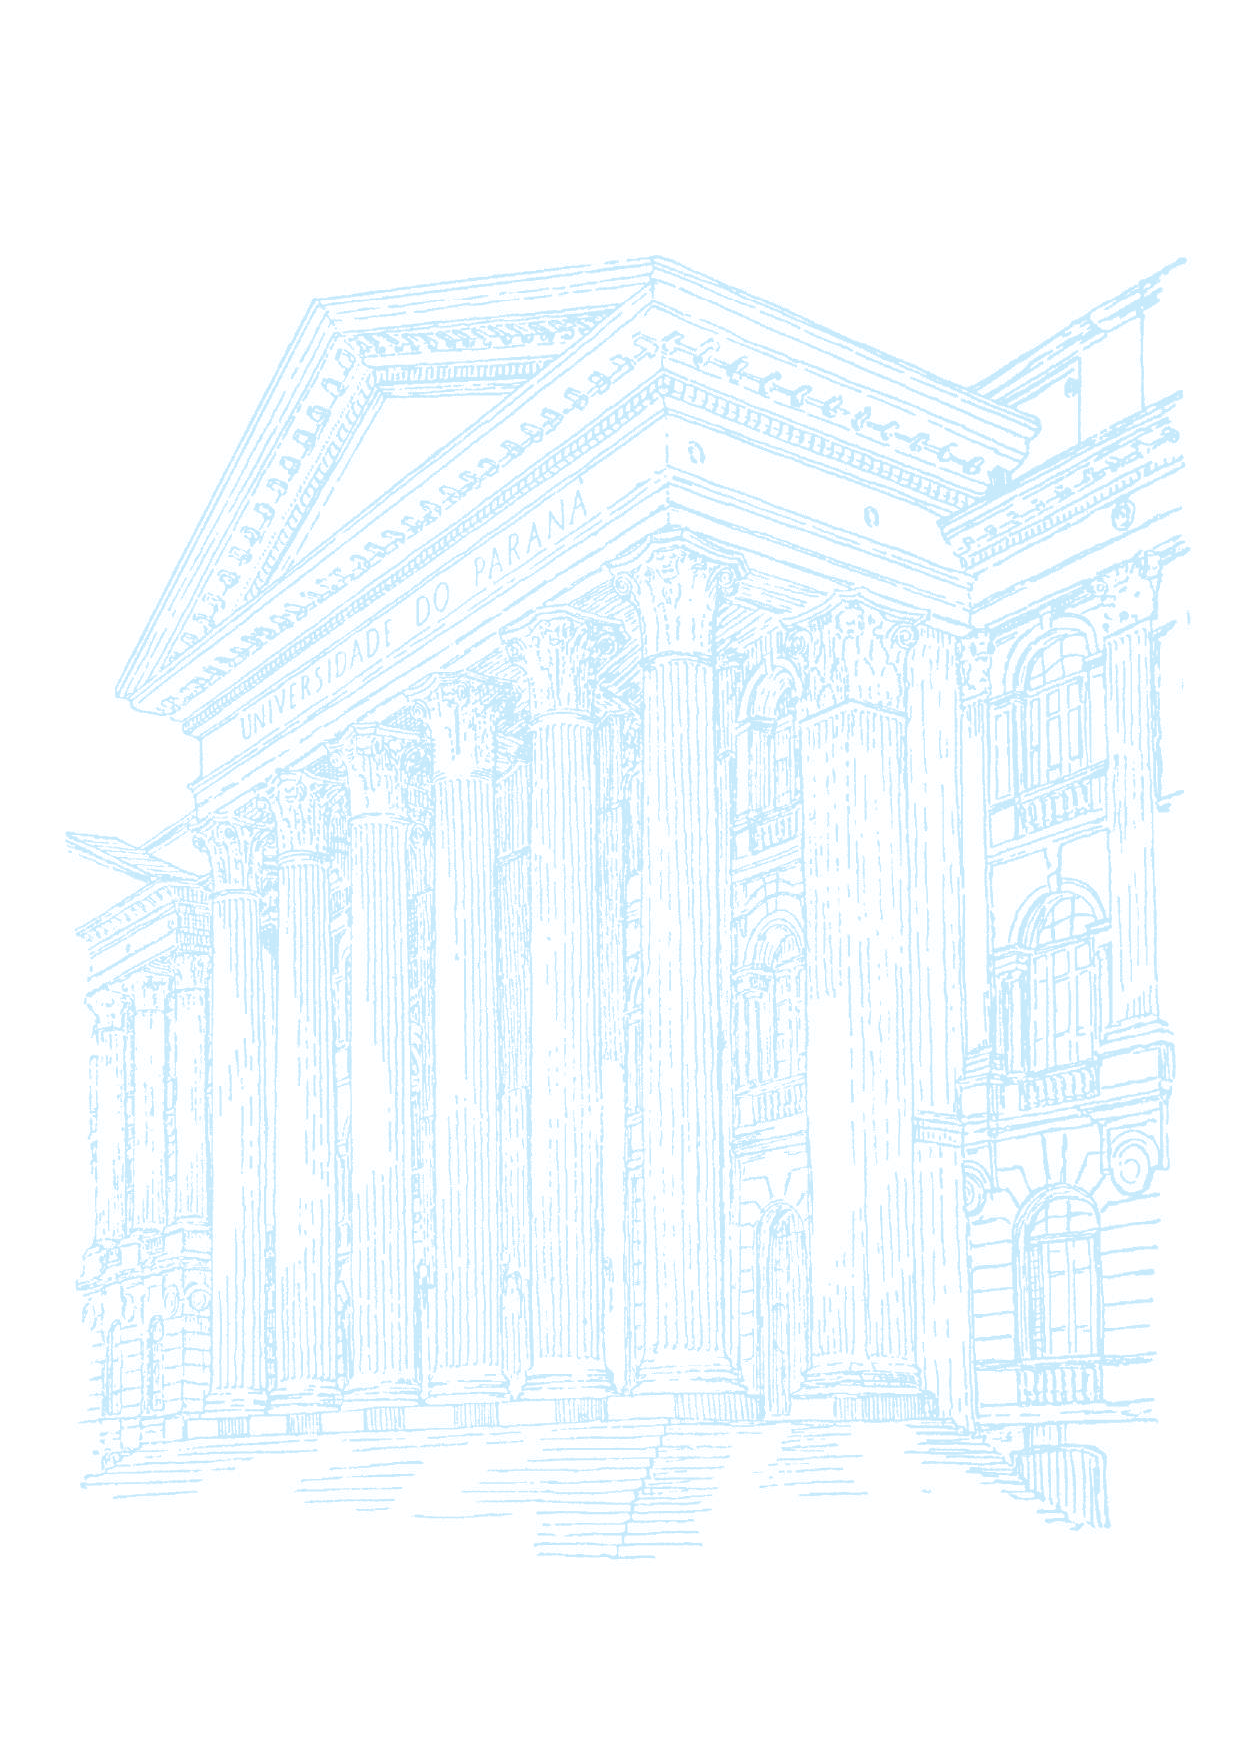
\includegraphics[width=\paperwidth,height=\paperheight]{imgs/UFPR.pdf}
\vfill
}}
}

\newcommand{\autoriapropria}{{\vspace{0.5cm} \centering\small Source: The author (2026).\par}}

% Arquivo de bibliografia
\addbibresource{bibfile.bib}
\setlength{\bibitemsep}{1\baselineskip}

% Margens
\usepackage{geometry}
\geometry{left=30mm,right=20mm,bindingoffset=0mm, top=30mm,bottom=20mm,includefoot}

% Imagens
\usepackage{graphicx}
\graphicspath{ {./imgs/} }

\usepackage{setspace}

\usepackage[labelfont=bf, singlelinecheck=false, format=hang]{caption}
\captionsetup{
    labelsep=endash,
    justification=justified
}

\usepackage{titlesec}
\usepackage{indentfirst}

\usepackage{fancyhdr}
\pagestyle{fancy}
\fancyhf{}
\renewcommand{\headrulewidth}{0pt}
\fancyhead[R]{\thepage}
\setlength{\headheight}{14.5pt}

\DeclareMathOperator{\sech}{sech}

\titleformat{\chapter}{\Large\bfseries\uppercase}{\thechapter}{1em}{}
\titleformat{\section}{\large\bfseries}{\thesection}{1em}{}
\titleformat{\subsection}{\fontsize{13pt}{15.6pt}\bfseries}{\thesubsection}{1em}{}


\titlespacing*{\section}{0pt}{12pt}{6pt}

\setlength\parindent{1.25cm}

\makeglossaries